\documentclass{article}  
\usepackage[margin=3cm]{geometry}
\usepackage{hyperref}
\usepackage{float}
\usepackage{listings}
\usepackage{graphicx}

\begin{document}  
  
\begin{center}
    {\Large {\bf Machine Learning in Agriculture}} \\
    \vspace{0.3cm}
    {\Large Literature Review} \\
    
    \vspace{1cm}
\end{center}

{\large {\bf Abstract}}

In this research project, we are trying to develop a method for Precision weeding in crop fields. Our initial step is to find the best approach to create a heatmap of the crops and weeds on the whole filed. Once we have such a map, we can feed it to a machine that is capable of spraying areas marked as weed in the field. There have been various approaches in detecting weeds in a crop filed. We will try to summarize many of those useful approaches here. \\

\section{Unsupervised Classification Algorithm for Early
Weed Detection in Row-Crops by Combining
Spatial and Spectral Information ~\cite{louargant-2018-mdpi-unsupervised}}
	
	This paper introduces an automatic approach in weed detection in order to reduce herbicide use in agriculture. They combine spatial and spectral information/features from four band multi spectral images. Images acquired using a camera mounted on a pole 3m above the ground. The automatic part of this method is as follows. They consider row crop arrangement as a ground truth in grouping the plants. In other words, everything not on the crop rows will be considered weed and things on the crop row might be either weed or plant. Then using these informations, a training dataset containing the multi-spectral image features is created and use to train a support vector machine (SVM). At the end for testing, inter-row crops are classified as weed (only based on spatial feature) and in-row crops are classified as either weed or crop using the SVM and the spectral features. They report 89 as their weed detection rate using the method mentioned earlier (combination of both spatial and spectral features), 79 for using only spatial features and 75 for using only spectral features. 
	
	\subsection{More on this method}
	
	One way to distinguish different approaches for detection and localization of weeds is the distance and the vehicle from which the images are captured which includes satellite, aerial, terrestrial vehicle, etc. Another one is the sensor used to capture images. Images can only have the three color bands (RGB) or might have other bands as well such as Near Infrared. One interesting approach is to use UAVs to capture multi-spectral images from large areas in a field. Based on the previous studies, weeds and crops can be discriminated using their reflectance spectra. However, there are some limitations: number of spectral bands is limited, field condition affects the spectral reflectance information, spectral reflectance changes with psychological stress. 
	
	At the time that this paper was written, the usual camera for weed detection on a UAV had 4 bands (near infrared + RGB). NIR helps separation of the vegetation and the background. 
	
	\subsection{Vegetation Indices}
	
	In most of the weed detection method, the first step is to distinguish the vegetation (whether it is weed or crop) from the background. It is usually done by calculating a Vegetation Index and applying a thresholding algorithm on that index value at each pixel. One of the most common indices is Normalized Difference Vegetation Index (NDVI) for the case where NIR data is available and Excess Green Index (ExG) when only RGB is available. 
	
	\subsection{Geometrical Information for weed detection}
	
	One approach for weed detection is to use geometrical information for detecting weeds. One is automatic row detection using textural based methods. People have used Gabor filters and Object-Based Image Analysis (OBIA) to detect the crop rows by segmentation. OBIA is something like a histogram of texture. 
	
	\subsection{Some Spatial and Spectral combination methods}
	
	There has been some methods that combined spatial and spectral features together using Bayesian methods and pixel neighborhood similarity. Another interesting method was using spatial information to detect inter-row weeds and then using some sort of nearest neighbor classifier with the vegetation index to classify in-row crops. Another method combined SVM and OBIA and reached 96 percent accuracy in sunflower fields. They also added a feature selection method which helped the accuracy. In some other methods, hough transform and randome forest are used which reached 96 percent accuracy. Another paper reconstructed the plants in 3D and used their average height to decide whether they are weed or crop. 
	
	In general, supervised classification is much better than unsupervised but it needs labeled training data. On the other hand, unsupervised methods can be used to generated labeled data. 
	
	\subsection{The proposed method in this paper}
	
	In the proposed method, they used a multi-spectral imaging system on a pole hold by a person who moves across the field. The sensors take 12 megapixel images in 550 (green), 660 (red), 735 (red-edge) and 790 (near-infrared) bands. The images were captured in a sunny day around noon. GPS was used to geo-tag the images. Images were taken every 1.5 meter which allows some overlap. There has been some preprocessing including color and illumination corrections.They proposed three different methods, one is based on spatial features only, another based on spectral features and the last one based on the combination of these two.
	
	\subsubsection{Spatial method}
	
	The algorithm proposed for this method uses the spatial information and some well-known image processing techniques to detect rows on which plants are sowed. It comprises of following steps:
	
	\begin{itemize}
		\item Using Fourier Transform to find the row orientation.
		\item Discerning Soil from Vegetation using NDVI index. 
		\item Using Hough Transform to detect lines that correspond to crop rows. The angle of the lines are limited to the orientation of the row which was calculated in the first step. Only the vegetation pixels are used.
		\item Finding the edges of the vegetations using connected components and linear regression on both sides of the row. 
		\item Crop and weed detection using a decision tree based on shape of the connected components. (axis orientation, area, etc.)
	\end{itemize}
	
\section{Combining computer vision and deep learning to enable ultra-scale aerial phenotyping and precision agriculture: A case study of lettuce production ~\cite{bauer-2019-combining-yield}}

This paper is discussing a novel Deep-Learning-based approach in analyzing yield-related crop phenotyping. They equipped fixed-wing light aircrafts with NDVI sensors to acquire the desired images. The platform which is called Airsurf-lettuce, is capable of scoring and categorizing iceberg lettuces with more than 98 percent accuracy. They trained their deep learning model using 100000 labeled lettuce signals. At the end, their platform is capable of producing a map of lettuce size (heat map) for detecting the areas that are ready for harvest. 

Growing lettuce is highly affected by the whether. Bad whether can cause reduction in the quantity as well as quality of the products. In average only 70-80 percent of planted lettuces will be used in the market. The goal of this paper is to use deep learning methods to find the best time for harvesting the crops.

In this paper they introduced Airsurf as an open source yield-related phenotyping analysis platform. In short, they capture NDVI images using NDVI sensors, then use CNNs to count crops in each image and other supervised ML techniques for assessing the quality of each individual crop. A customized and commercialized version of Airsurf (Airsurf-Lettuce) is used for lettuce. 

\subsection{Material and Methods}

\subsubsection{Normalized Difference Vegetation Index (NDVI)}
NDVI is a well-known index which is widely used to discern between vegetation and non-vegetation areas in an image usually from a field or a forest. It is used to determine how dense vegetation is in an area. According to biologists, plants re-emit solar radiation in the Near-Infrared spectral (NIR) due to the fact that those radiations do not have enough energy to be used in photosynthesis and only result in overheating the plants if absorbed. Therefore, plants are relatively bright in NIR band. On the other hand, snow, clouds and other materials are relatively dark in NIR but relatively bright in Red spectral band. Scientists have been using these facts to define a vegetation index using the following formula:

\begin{eqnarray*}
	NDVI = \frac{NIR - RED}{NIR + RED}
\end{eqnarray*}

This is called Normalized Difference Vegetation Index or NDVI. It is usually between -1 and 1 but most of the surfaces on earth produce a number between 0 and 1. An NDVI close to 1 shows a dense vegetation at that specific area in an image. 

Due to the usefulness of this index, there has be NDVI cameras developed in the past years. In this paper, they equipped their light aircraft with such a camera which were able to capture NDVI images at the height of around 300m (1000 feet) when the aircraft was flying with a speed of 180 to 200 km/h. The farmers regularly capture NDVI images 4-5 times each season. Each image is 1.5 - 2 GB in size. They used the acquired images of one field to train the models. For validating the final model, farmers counted all the crops in that specific field manually and labeled some randomly chosen lettuces for quality assessment phase. 

\subsubsection{The dataset}

From the NDVI images acquired, they randomly selected 60 subsections each containing between 300 and 1000 lettuce heads. Then they labeled them using 20 by 20 pixel bounding boxes. Then a balanced training dataset of 100000 patches of size 20 by 20 were created to train a CNN for classifying lettuce vs non-lettuce. Then a non-overlapping slide window were applied over the images to separate foreground and background using this CNN. Note that training and testing sets were balanced and a validation set is used to avoid overfitting of the network. 

\subsubsection{The analysis workflow of the platform}

The following image summarizes the workflow of the proposed method. 

\begin{figure}[H]
	\begin{center}
		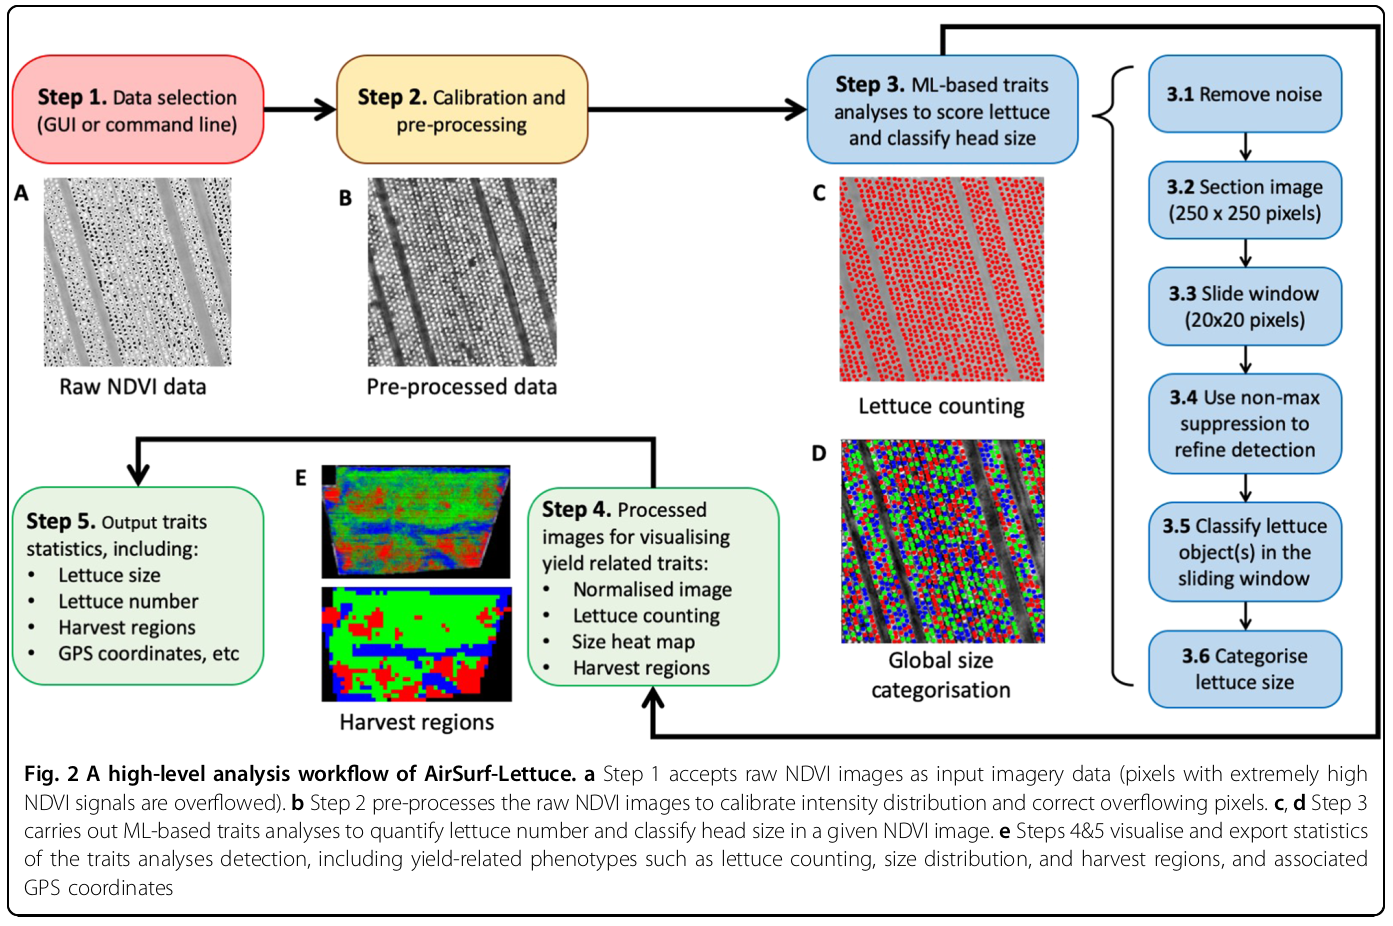
\includegraphics[width=14cm]{img/1}
	\end{center}
\end{figure}
	
In the second step, a histogram equalization algorithm is used to increase the contrast between lettuces and the background. The algorithm is called CLAHE. In the third step, each image first is divided into 250X250 size sections and then a 20 by 20 window is traversed over these sections to detect and count lettuces. A non-maximum suppression is also used. For each lettuce its size is then detected and reported back to the user in a csv file. The whole platform has a GUI which makes things easier for users. 

\subsubsection{The Neural Network Architecture}

The Neural Network which was used to classify 20 by 20 patches into lettuce/non-lettuce signals has a deep architecture similar to AlexNet. However, they did not use any pre-trained networks and they train it from scratch based on the paper. The structure of the network comprises of 4 blocks of convolution layers plus a fully connected layer at the end of the network. It seems that the activation function for the last layer is sigmoid. Their network was trained on the training data for 10 epoch (stopped using validation set). 

\subsubsection{Size Categorization Algorithm}

For size categorization, they have used an unsupervised approach. They create a histogram and put the NDVI pixel values in 20 by 20 patches into 10 bins. Then using these histograms and k-means algorithm, they put the patches into 3 different clusters. Then by calculating the dot product between the histogram values and bin number (pixel intensity), they determine which cluster is small, which is medium and which is large. 

\subsubsection{Improvement for the CNN Classifier}

To improve the efficiency of the detection and counting algorithm, they first divide the big NDVI images into 250 by 250 sections and then run the sliding window technique on that. Moreover, they use a non-maximum suppression technique when doing the sliding window to avoid counting any lettuces for two times. They also manually labeled another 500 lettuces in the very bright or dark areas and re-train the network. 

\subsubsection{GPS-tagged Harvest map}

In the next step, a distribution map of lettuce sizes is generated. Then each field is gridded based on geographical features and GPS information and each cell of the grid is colored with the most representative size category of the lettuce in that cell. This is how the harvest map is generated. This can be used by the farmers to find the regions on each field that are ready for harvest. A 3D bar plot is also generated that shows the distribution of the lettuces in terms of their size and number for each cell of the grid. 

\subsubsection{Validation of counting algorithm}

For validating the counting algorithm they tested Airsurf-L on three different fields in UK. They divided the fields into three different region types: Small regions with less than 400 lettuces, Large regions with greater than 900 lettuces and mixed regions with variety number of lettuces in it. The R-squared correlation between human counting the lettuces and Airsurf results for small regions, large regions and mixed regions were 0.978, 0.988 and 0.9997 respectively. R-squared is calculated using the following formula:

\begin{eqnarray*}
R^2 = 1-\frac{\sum_{i=1}^{n}(y_i -f_i)^2}{\sum_{i=1}^{n}(y_i -\bar{y})^2}
\end{eqnarray*}

\subsubsection{Future Thoughts and My Ideas}

It is mentioned in the paper that we can add other features such as weather change and soil phenotype information to better predict the harvest time. I was thinking of predicting the heatmap in a time line using a combination of ML and DL methods. It is also possible to use this platform on other crops such as wheat and rice. 

\section{Canopeo: A Powerful New Tool for Measuring Fractional
Green Canopy Cover ~\cite{patrignan-2015-canopeo}}

This paper introduces a tool for estimating the canopy coverage of different plants, called "Canopeo". The corresponding author is an associate professor at the plants and soil sciences department at the Oklahoma State University. They have developed android and IOS applications for their tool as well. In the following paragraphs, I will include some details about their method and their developed applications.

\subsection{Previous Works}
In this section, I will include useful information I retrieved related to the previous works mentioned in the paper. I also saved some interesting papers for further reading. \\

Apparently there are two methods for canopy cover estimation: Manual Pixel Classification (MPC) and Automatic Color Threshold (ACT). In the first one, for each image a set of about 200 random pixels is given to an expert for manual classification (vegetation or soil) and then other pixels are classified based on this. SamplePoint is a software that uses this method. On the other hand, in the second method, threshold values are specified by the user and then used to classify image pixels. SigmaScan is an software that uses this method. It is used to analyze canopy cover and light interception in soybean. These two softwares were reported to be slow and only appropriate for small images. \\

FGCC is short form of Fractional Green Canopy Cover. Alongside with other indexes such as NDVI, Crop Height and LAI (leaf area index) can be used in many applications in the plant science field. 

\subsection{Canopeo, The Methodology}

This software uses an ACT method and works with RGB images. In short, it uses R/G and B/G ratios and also Excess Green Index ($2G - R - B$). The pixels of the binary result image is calculated using the formula below:

\begin{eqnarray}
\left\{
	\begin{array}{ll}
		1  & \mbox{if } \frac{R}{G} < P_1 \;\;AND\;\; \frac{B}{G} < P_2 \;\;AND\;\; 2G - R - B > P_3 \\
		0 & \mbox{ } otherwise
	\end{array}
\right.
\end{eqnarray}

where $P_1, P_2$ are parameters with values near 1 that classify pixels that are in the green band. $P_3$ is a parameter that sets the minimum excess green index which is fixed to 20. Excess green index is useful for classifying dark or gray pixels that can not be classified using the other two ratios. By analyzing connected neighboring pixels, Canopeo can remove some noise too. \\

These were all relevant details regarding the methodology of this tool. Other informations in the paper are related to discussion. The way they compared their method didn't catch my attention. I don't consider this paper very useful to our task. On the other hand the next paper seems more interesting. \\

\section{Unmanned aerial vehicle (UAV) derived structure-
from-motion photogrammetry point clouds for oil
palm (Elaeis guineensis) canopy segmentation and
height estimation ~\cite{fawcett_uav_2019_canopy}}


\section{Ultra-fine grain landscape-scale quan-
tification of dryland vegetation structure with drone-acquired structure-from-motion photogrammetry ~\cite{cunliffe-2016-ultra}}

\section{4D crop monitoring: Spatio-temporal reconstruction for agriculture ~\cite{dong-2017-4d}}

In this paper, they tackled the problem of estimating the 3D structure of plants (peanut in this case) over time. They call their method, spatio-temporal reconstruction. They represent the plant 3D structure using 3D point clouds. So, they produce a 3D point cloud for each time frame. In short, they follow the pipeline below:

\begin{itemize}
\item[1.] Extracting feature points (SIFT) and keep those that have high number of matching between consecutive image frames. (using RANSAC and nearest neighbor).
\item[2.] Estimating camera states including translation, rotation, and so on by creating a factor graph for each row and each session of imaging. This is done by optimizing a factor graph. After having the camera states, they generate a point cloud for each row and session. 
\item[3.] Doing data association over time using a robust method. They use two methods for associating feature points from different rows and different time to each other. They find a good way of associating different points in the point cloud to each other. The first method is called back projection bound search. In that they bound the search area for finding the association by defining a bounding box around the feature points. This is a way of eliminating outliers. Second, they homography to associate feature points to each other from different time sessions. 
\item[4.] The last step is 4D reconstruction which is done again by using a factor graph and optimizing it. In the final stage, they have a sequence of point clouds. 
\end{itemize}

They gathered their own dataset from a peanut field in GA. In evaluating their method, they measure two different things. First is to measure whether the point cloud is objectively aligned in the space or not (comparing to the ground truth). For this, compare their method with another method visually. For the second measurement, the calculate the RMS error between an estimated plant property like canopy height and the ground truth gathered by humans. They reported a 2.93 cm RMSE for plant height. 

\section{Branching Gaussian Processes with Applications to Spatiotemporal Reconstruction of 3D Trees ~\cite{simek-2016-branching}}

\section{Inferring Grammar-based Structure Models from 3D Microscopy Data ~\cite{schlecht-2007-inferring}}

\section{Gaussian Process Shape Models forBayesian Segmentation of Plant Leaves ~\cite{simek-2015-gaussian}}




\bibliographystyle{plain}
\bibliography{Agriculture_Literature_Review}
	
\end{document}